\documentclass{assignment}
\UsingEnglish
\ProjectInfos*{Intro to Communication System}{EE140}{Fall, 2020}{Assignment 8}{Due time : 10:15, Nov 27, 2020 (Friday)}{陈稼霖}{45875852}
\begin{document}
\begin{prob}[2.11]
    Proof of the Kraft inequality for uniquely decodable codes.
    \begin{itemize}
        \item[(a)] Assume a uniquely decodable code has lengths $l_1,\cdots l_M$. In order to show that $\sum_j2^{-l_j}\leq 1$, demonstrate the following identity for each integer $n\geq 1$:
        \[
            \left[\sum_{j=1}^M2^{-l_j}\right]^n=\sum_{j_1=1}^M\sum_{j_2=1}^M\cdots\sum_{j_n=1}^M2^{-(l_{j_1}+l_{j_2}+\cdots l_{j_n})}.
        \]
        \item[(b)] Show that there is one term on the right for each concatenation of $n$ codewords (i.e. for the encoding of one $n$-tuple $\bm{x}^n$) where $l_{j_1}+l_{j_2}+\cdots+l_{j_n}$ is the aggregate length of that concatenation.
        \item[(c)] Let $A_i$ be the number of concatenations which have overall length $i$ and show that
        \[
            \left[\sum_{j=1}^M2^{-l_j}\right]^n=\sum_{i=1}^{nl_{max}}A_i2^{-i}.
        \]
        \item[(d)] Using the unique decodablility, upperbound each $A_i$ and show that
        \[
            \left[\sum_{j=1}^M2^{-l_j}\right]^n\leq nl_{\max}.
        \]
        \item[(e)] By taking the $n$th root and letting $n\rightarrow\infty$, demonstrate the Kraft inequality.
    \end{itemize}
\end{prob}
\begin{pf}
    \begin{itemize}
        \item[(a)] 
        \begin{align}
            \left[\sum_{j=1}M2^{-l_j}\right]^n=\left[\sum_{j_1=1}^M2^{-l_{j_1}}\right]\left[\sum_{j_2=1}^M2^{-l_{j_2}}\right]\cdots\left[\sum_{j_n=1}^M2^{-l_{j_n}}\right]=\sum_{j_1=1}^M\sum_{j_2=1}^M\cdots\sum_{j_n=1}^M2^{-(l_{j_1}+l_{j_2}+\cdots+l_{j_n})},\quad\forall n\geq 1.
        \end{align}
        \item[(b)] For each concatenation of $n$ codewords $\bm{x}^n$, the length of the $k$th codeword is $l_{j_k}$ and there is $n$ codewords in total ($1\leq k\leq n$), so the aggregate length of the concatenation is $l_{j_1}+l_{j_2}+\cdots+l_{j_n}$.
        \item[(c)] Using the conclusion we obtained in (b), we have
        \begin{align}
            \left[\sum_{j=1}^M2^{-l_j}\right]^n=\sum_{\bm{x}^n}e^{-(\text{length of }\bm{x}^n)}=\sum_{i=1}^{nl_{\max}}A_i2^{-i}.
        \end{align}
        \item[(d)] Because of unique decodablility (i.e. each concatenation should be different),
        \begin{align}
            A_i\leq 2^i,\quad\forall i.
        \end{align}
        Thus,
        \begin{align}
            \label{P-1-d}
            \left[\sum_{j=1}^M2^{-l_j}\right]^n=\sum_{i=1}^{nl_{\max}}A_i2^{-i}\leq\sum_{i=1}^{nl_{\max}}2^i2^{-i}=\sum_{i=1}^{nl_{\max}}1=nl_{\max}.
        \end{align}
        \item[(e)] Taking the $n$th root of equation \eqref{P-1-d}, we have
        \begin{align}
            \sum_{j=1}^M2^{-l_j}\leq[nl_{\max}]^{1/n}.
        \end{align}
        Letting $n\rightarrow\infty$, we have
        \begin{align}
            \sum_{j=1}^M2^{-l_j}\leq\lim_{n\rightarrow\infty}[nl_{\max}]^{1/n}=1,
        \end{align}
        which is the Kraft inequality.
    \end{itemize}
\end{pf}

\begin{prob}[2.12]
    A source with an alphabet size of $M=\abs{\mathcal{X}}=4$ has a symbol probabilities $\{1/3,1/3,2/9,1/9\}$.
    \begin{itemize}
        \item[(a)] Use the Huffman algorithm to find an optimal prefix-free code for this source.
        \item[(b)] Use the Huffman algorithm to find another optimal prefix-free code with a different set of lengths.
        \item[(c)] Find another prefix-free code that is optimal but cannot result from using the Huffman algorithm.
    \end{itemize}
\end{prob}
\begin{sol}
    \begin{itemize}
        Suppose the four symbols corresponding to the probabilities $\{1/3,1/3,2/9,1/9\}$ are a,b,c,d.
        \item[(a)] An optimal prefix-free code for this source is shown in figure \ref{A-8-P-2-a}.
        \item[(b)] Another optimal prefix-free code for this source is shown in figure \ref{A-8-P-2-b}.
        \begin{figure}[h]
            \centering
            \subfigure[An optimal prefix-free code derived from the Huffman algorithm]{
                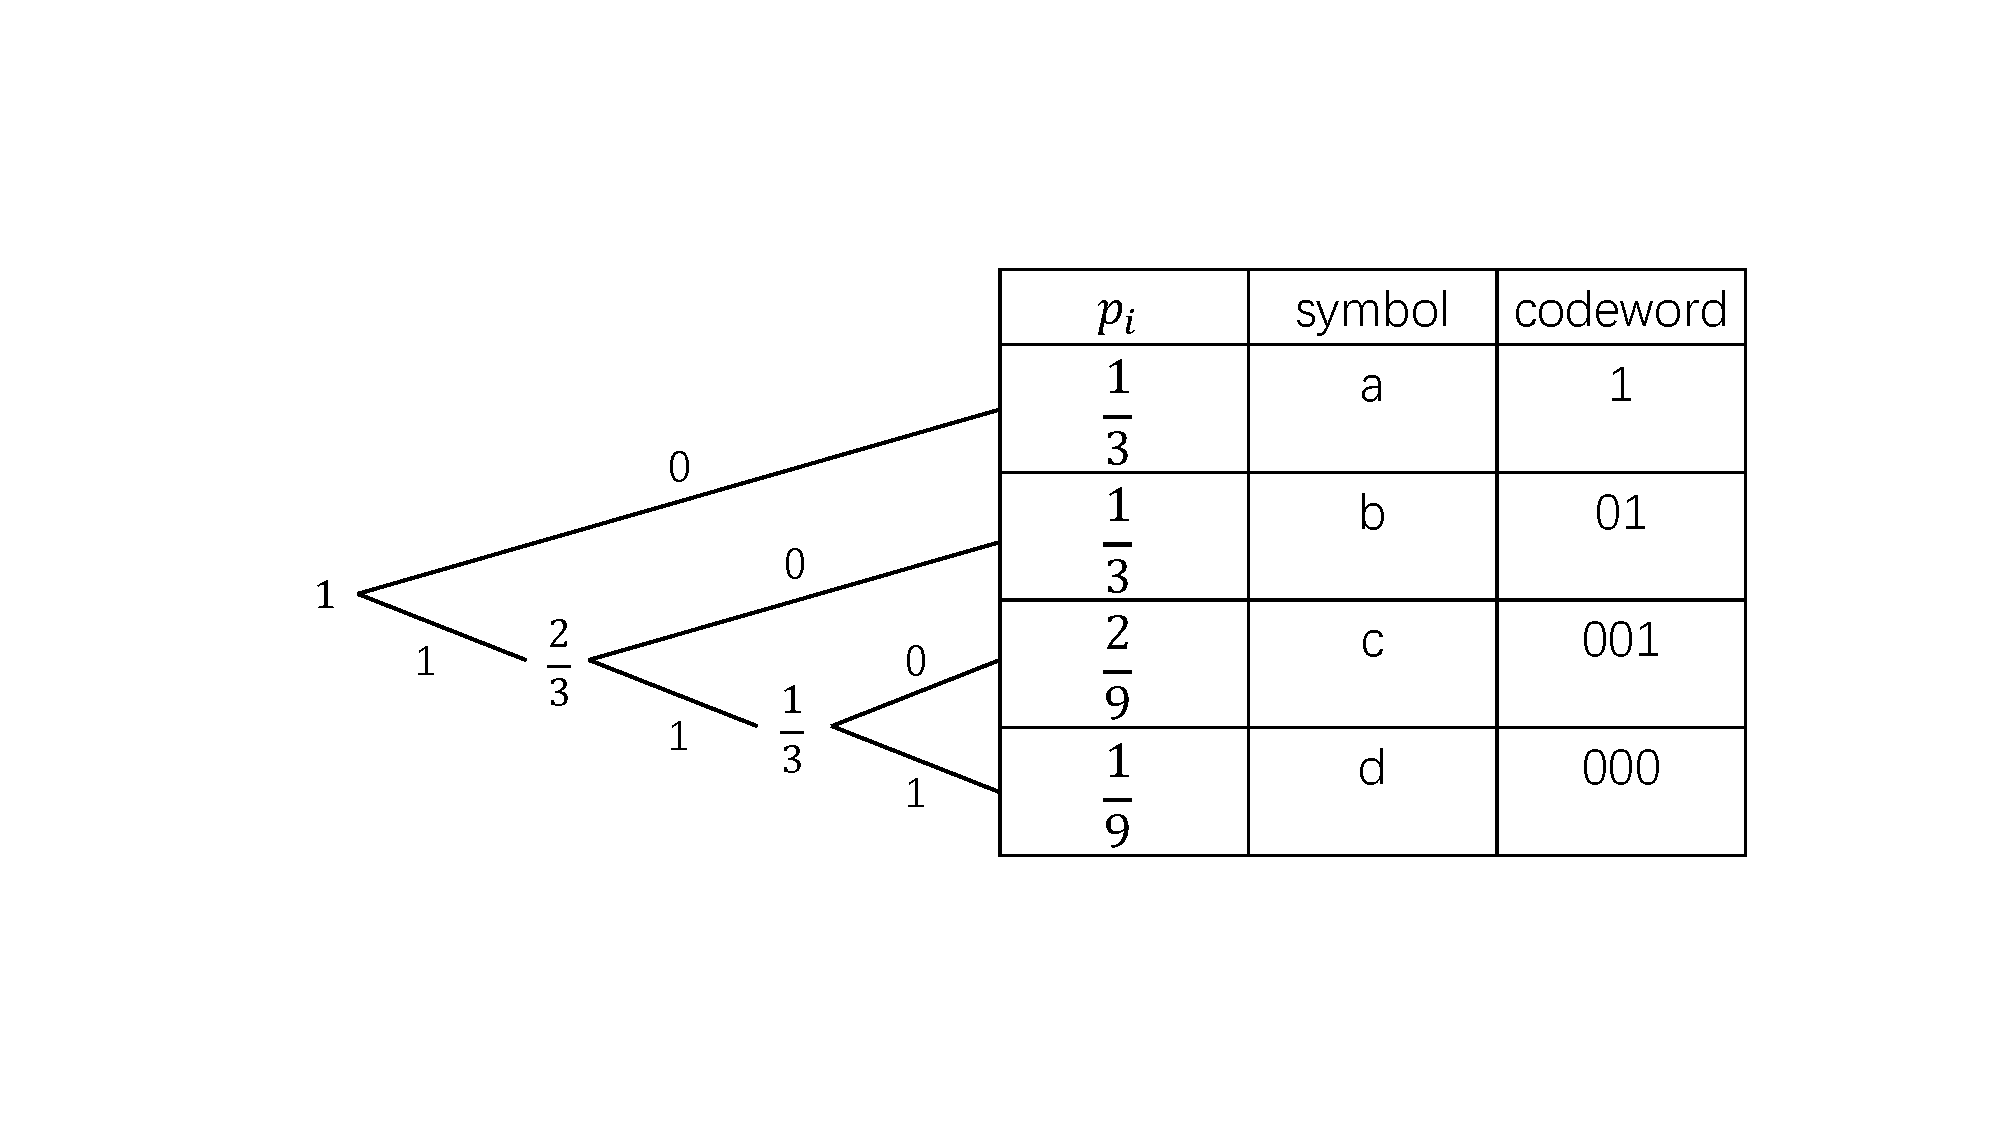
\includegraphics[width=.45\columnwidth]{A-8-P-2-a.pdf}
                \label{A-8-P-2-a}
            }
            \subfigure[Another optimal prefix-free code derived from the Huffman algorithm]{
                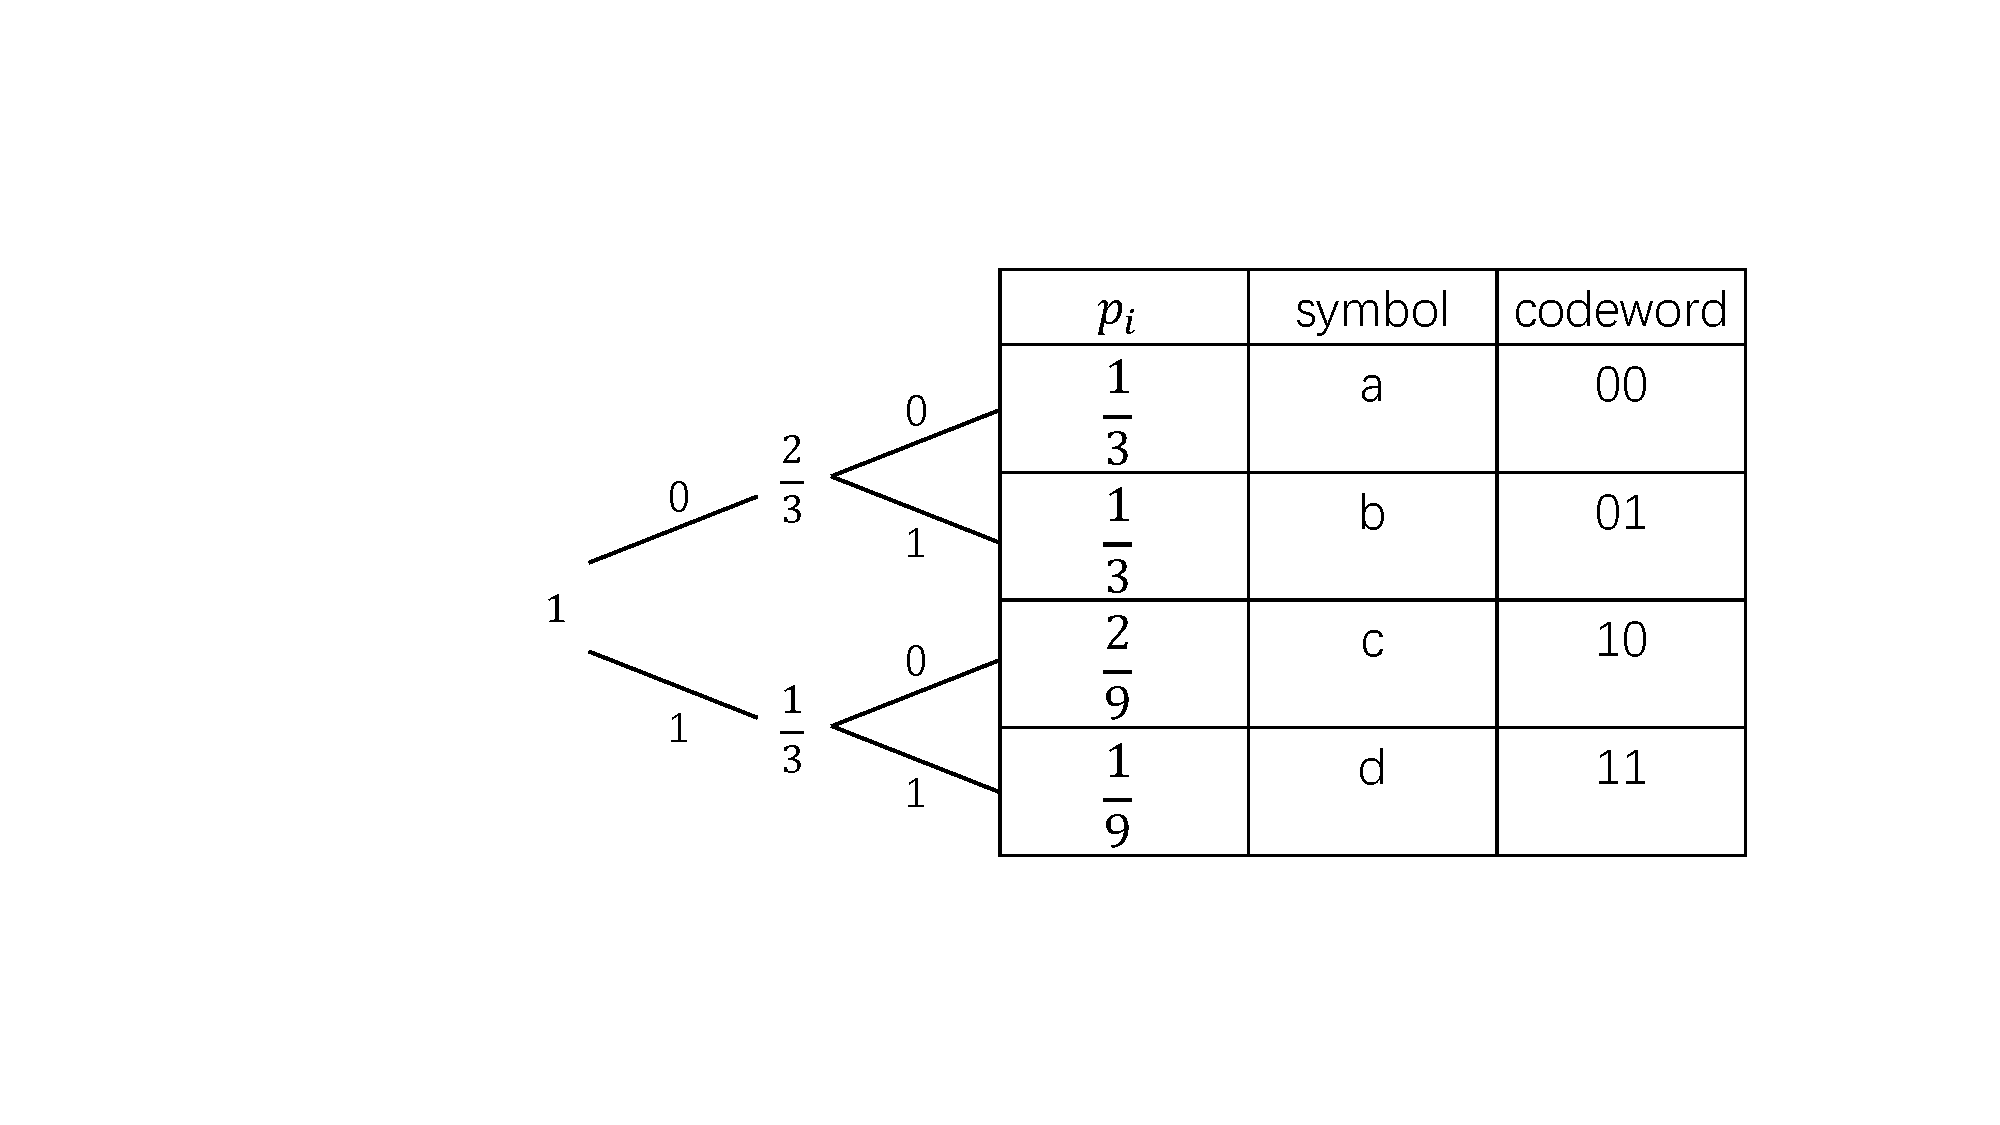
\includegraphics[width=.45\columnwidth]{A-8-P-2-b.pdf}
                \label{A-8-P-2-b}
            }
            \item[(c)] Another prefix-free code that is optimal but cannot result from using the Huffman algorithm is shown in table \ref{A-8-P-2-c}.
            \begin{table}[H]
                \centering
                \caption{Another prefix-free code that is optimal but cannot result from using the Huffman algorithm}
                \label{A-8-P-2-c}
                \begin{tabular}{|c|c|}
                \hline
                symbol & codeword \\ \hline
                a & 00 \\ \hline
                b & 11 \\ \hline
                c & 10 \\ \hline
                d & 01 \\ \hline
                \end{tabular}
                \end{table}
        \end{figure}
    \end{itemize}
\end{sol}

\begin{prob}[2.14]
    Consider a source with $M$ equiprobable symbols.
    \begin{itemize}
        \item[(a)] Let $k=\lceil\log M\rceil$. Show that, for a Huffman code, the only possible codeword lengths are $k$ and $k-1$.
        \item[(b)] As a function of $M$, find how many codewords have length $k=\lceil\log M\rceil$. What is the expected codeword length $\bar{L}$ in bits per source code?
        \item[(c)] Define $y=M/2^k$. Express $\bar{L}-\log M$ as a function of $y$. Find the maximum value of this function over $1/2<y\leq 1$. This illustrates that the entropy bound, $\bar{L}=H[X]+1$, is rather loose in this equiprobable case.
    \end{itemize}
\end{prob}
\begin{sol}
    \begin{itemize}
        \item[(a)] For a Huffman code, if $M$ is a power of $2$, say $M=2^k$, then the Huffman tree should be a full binary tree and the length is $k=\log_2M$ for all codewords. If $M$ is not a power of $2$, say $M=2^{k-1}+k_0$ where $0<k_0\leq 2^{k-1}$, the Huffman tree should be a complete but not full binary tree. In this case, some codewords are at the bottom layer of the Huffman tree whose lengths are all $k=\lceil\log_2M\rceil$, other codewords are at the bottom but one layer whose lengths are all $k-1=\lceil\log_2M\rceil-1$.
        \item[(b)] Suppose the number of codewords with length $k$ is $x$, then the number of codewords with length $k-1$ is $M-x$. The number of node at the bottom but one layer of the Huffman tree should be
        \begin{align}
            \frac{x}{2}+(M-x)=2^{k-1},
        \end{align}
        so the number of codeword with length $k$ is
        \begin{align}
            x=2M-2^k.
        \end{align}
        The expected code length per source code is
        \begin{align}
            \bar{L}=\frac{k(2M-2^k)+(k-1)(2^k-M)}{M}=k+1-\frac{2^k}{M}.
        \end{align}
        \item[(c)] Using $k=\log_2\frac{M}{y}$, we have
        \begin{align}
            \bar{L}-\log_2M=-\log_2y+1-\frac{1}{y}.
        \end{align}
        The derivative of the above function is
        \begin{align}
            \frac{\mathrm{d}}{\mathrm{d}y}=-\frac{1}{y\ln 2}+\frac{1}{y^2}\left\{\begin{array}{ll}
                >0,&\frac{1}{2}\leq y<\ln 2,\\
                <0,&\ln 2<y<1,
            \end{array}\right.
        \end{align}
        so the maximum value of the above function is
        \begin{align}
            \left[\bar{L}-\log_2M\right]_{\max}=\left[\bar{L}-\log_2M\right]_{y=\ln 2}=-\log_2(\ln 2)+1-\frac{1}{\ln 2}=0.086,
        \end{align}
        which means that
        \begin{align}
            \bar{L}\leq\log_2M+0.086\leq H(X)+0.086.
        \end{align}
        Therefore, the entropy bound $\bar{L}=H[X]+1$, is rather loose in this equiprobable case.
    \end{itemize}
\end{sol}

\begin{prob}[2.21]
    A discrete memoryless source emits iid random symbols $X_1,X_2,\cdots$ Each random symbol $X$ has the symbols $\{a,b,c\}$ with probabilities $\{0.5,0.4,0.1\}$, respectively.
    \begin{itemize}
        \item[(a)] Find the expected length $\bar{L}_{\min}$ of the best variable-length prefix-free code for $X$.
        \item[(b)] Find the expected length $\bar{L}_{\min,2}$, normalized to bits per symbol, of the best variable-length prefix-free code for $X^2$.
        \item[(c)] Is it true that for any DMS, $\bar{L}_{\min}\geq\bar{L}_{\min,2}$? Explain your answer.
    \end{itemize}
\end{prob}
\begin{sol}
\end{sol}

\begin{prob}[2.33]
    Perform an LZ77 parsing of the string \uline{00011101}0010101100. Assume a window of length $W=8$; the initial window is underlined above. You should parse the reset of the string using the Lempel-Ziv algorithm.
\end{prob}
\begin{sol}
\end{sol}

\begin{prob}[4.35 Aliasing]
    The following exercise is designed to illustrate the sampling of an approximately baseband waveform. To avoid messy computation, we look at a waveform baseband-limited to $3/2$ which is sampled at rate $1$ (i.e. sampled at only $1/3$ the rate that it should be sampled at). In particular, let $u(t)=\sinc(3t)$.
    \begin{itemize}
        \item[(a)] Sketch $\hat{u}(f)$. Sketch the function $\hat{v}_m(t)=\rect(f-m)$ for each integer $m$ such that $v_m(f)\neq 0$. Note that $\hat{u}(f)=\sum_m\hat{v}_m(f)$.
        \item[(b)] Sketch the inverse transforms $v_m(t)$ (real and imaginary parts if complex).
        \item[(c)] Verify directly from the equations that $u(t)=\sum v_m(t)$. [Hint. This is easier if you express the sine part of the sinc function as a sum of complex exponentials.]
        \item[(d)] Verify the sinc-weighted sinusoid expansion, (4.73). (There are only three nonzero terms in the expansion.)
        \item[(e)] For the approximation $s(t)=u(0)\sinc(t)$, find the energy in the difference between $u(t)$ and $s(t)$ and interpret the terms.
    \end{itemize}
\end{prob}
\begin{sol}
\end{sol}
\end{document}